%
% general.tex -- XXX
%
% (c) 2019 Prof Dr Andreas Mueller
%
\section{Der allgemeine Fall}
Wir möchten jetzt den allgemeinen Fall des Problems
\begin{align*}
\Delta u&=f&&\text{in $\Omega$}\\
u&=g&&\text{auf $\partial\Omega$}
\end{align*}
mit Hilfe einer Integralformel der Art (\ref{greenformula}) 
lösen. Nach dem Muster des eindimensionalen Falles suchen
wir eine partikuläre Lösung $G(x,\xi)$ für eine spezielle rechte Seite,
nämlich eine Delta-Funktion im Punkt $\xi$.  Hat man eine
solche, kann man auch die Lösung für ein beliebiges $f$ mit
Hilfe eines Integrals finden.


\subsection{Eine partikuläre Lösung}
\rhead{Partikuläre Lösung}
Das eindimensionale Musterproblem suggeriert, dass es eine
Funktion $\sigma(x,\xi)$ gibt, mit welcher eine partikuläre Lösung
der Laplace-Gleichung mittels des Integrals
\begin{equation}
u_p(x)=\int_\Omega \sigma(x,\xi)  f(\xi)\,d\xi
\label{singulaereloesunglaplace}
\end{equation}
gefunden werden kann.
Diese partikuläre Lösung muss die Randbedingungen nicht erfüllen,
sondern nur die Gleichung $\Delta u=f$.

Die Funktion $\sigma$ hängt, da sie auf die Randbedingungen nicht 
Rücksicht nehmen muss, nicht von $\Omega$ ab, sondern nur von der
Dimension $n$.
Wählt man für $f$ eine $\delta$-Funktion im Punkt $y$, folgt
\[
u(x)
=
\int_\Omega \sigma(x,\xi)\delta(\xi - y)\,d\xi
=
\sigma(x,y).
\]
Die Funktion $x\mapsto \sigma(x,y)$ erfüllt also die Gleichung
$\Delta \sigma(x,y)=0$ für alle Punkte von ${\mathbb R}^n\setminus\{y\}$.
Die Funktion $\sigma$ muss also eine harmonische Funktion in 
$\mathbb R^n\setminus\{y\}$ sein.

Die Bestimmung der Funktionen $\sigma(x,y)$ ist etwas mühsam, und wir
geben hier nur das Resultat an.
Man findet,\footnote{Man kann
diese Lösungen mit folgendem Argument finden. Zunächst darf die Lösung
nur von der Entfernung $|x-\xi|$ abhängen, so dass wir ohne
Beschränkung der Allgemeinheit $\xi=0$ annehmen dürfen.
Da $\Delta u=\operatorname{div}\operatorname{grad}u$ gilt folgt mit
dem Satz von Gauss
\begin{align*}
1&=\int_{B_r^n} \Delta u(x)\,d\mu(x)
=
\int_{B_r^n} \operatorname{div}\operatorname{grad} u(x)\,d\mu(x)
=\int_{S_r^{n-1}}\operatorname{grad}u(x)\cdot dn
\\
&=\int_{S_r^{n-1}}|\operatorname{grad}u(x)|\,d\mu(x)
=\mu(S_r^{n-1})\left|\frac{d}{dr}u(r)\right|
\\
\Rightarrow\qquad\frac{d}{dr}u(r)
&=\frac1{\mu(S_r^{n-1})}
=\frac1{\mu(S_1^{n-1})r^{n-1}}.
\end{align*}
Für $n=2$ ist $\mu(S_r^1)=2\pi r$, also
\[
u'(r)=\frac1{2\pi r}\quad\Rightarrow\quad u(r)=\frac1{2\pi}\log|r|.
\]
Für $n\ge 3$ gilt
\[
u'(r)=\frac1{\mu(S^{n-1})}r^{1-n}\quad\Rightarrow\quad u(r)=\frac1{\mu(S^{n-1})}\cdot \frac1{2-n}r^{2-n}.
\]
} und für $n=1$ haben wir diese Funktion ja schon in (\ref{n1sigma})
gefunden,
als Lösung
\begin{equation}
\sigma(x,\xi)=
\begin{cases}
\displaystyle \frac12|x-\xi|
&\qquad \text{für $n=1$}
\\
\\
\displaystyle \frac1{2\pi}\log|x-\xi]
&\qquad \text{für $n=2$}
\\
\\
\displaystyle -\frac1{4\pi}\frac1{|x-\xi|}
&\qquad \text{für $n= 3$}
\\
\\
\displaystyle \frac1{(2-n)\mu(S^{n-1})}|x-\xi|^{2-n}
&\qquad \text{für $n\ge 3$}
\end{cases}
\end{equation}
Durch etwas langweiliges Ausrechnen der Ableitungen kann man verifizieren,
dass diese Funktionen tatsächlich Lösungen sind, und dass
(\ref{singulaereloesunglaplace}) eine partikuläre Lösung der
Laplace-Gleichung ist.

\subsection{Greensche Funktion}
\rhead{Greensche Funktion}
Die vorgeschlagenen $\sigma$ sind nicht die einzigen für die die
Formel (\ref{singulaereloesunglaplace}) eine partikuläre Lösung ergibt.
Addiert man zu $\sigma$ eine beliebige Funktion $h(x,\xi)$, die
also Funktion von $x$ harmonisch ist, dann ist
\[
u(x)=\int_{\Omega}\sigma(x,\xi)f(\xi)\,d\xi-\int_{\Omega}h(x,\xi)f(\xi)\,d\xi
\]
ebenfalls eine Lösung von (\ref{elliptisch:laplaceequation}). Insbesondere
könnten wir $h(x,\xi)$ so wählen, dass
$x\mapsto h(x,\xi)$ eine Lösung des Randwertproblems
\begin{align*}
\Delta_x h(x,\xi)&=0&&x\in\Omega\\
h(x,\xi)&=\sigma(x,\xi)&&x\in\partial\Omega
\end{align*}
ist.
Die Funktion $h$ hat als die gleichen Randwerte wie $\sigma$.
Dann ist $\sigma(x,\xi)-h(x,\xi)$ eine Funktion, die auf dem
Rand $\partial\Omega$ immer verschwindet.
Die mittels
(\ref{singulaereloesunglaplace}) gefundene Lösung $u(x)$
verschwindet ebenfalls auf dem Rand.
%\marginpar{\tiny Greensche Funktion für das Dirichletproblem auf $\Omega$}
Wir bezeichnen $\sigma-h$ für diese spezielle Wahl von $h$ mit
\[
G(x,\xi)=\sigma(x,\xi)-h(x,\xi)
\]
und nennen sie die Greensche Funktion für das Dirichlet Problem.

\begin{satz}Ist $\Omega$ ein Gebiet, auf dem das Dirichlet-Problem
eindeutig lösbar ist, dann gibt es eine 
Funktion $G(x,\xi)$,
welche als Funktion von $x$ die Gleichung
\[
\Delta G(x,\xi)=\delta(x-\xi)
\]
löst mit homogenen Randbedingungen.
\end{satz}

Man beachte, dass dieser Satz zwar die Existenz einer Greenschen Funktion
garantiert, aber keinen Hinweis gibt, wie sie berechnet werden kann.
Die Greensche Funktion hängt aber nur vom Gebiet ab, nicht von den
Randbedingungen.
Da es Gebiete gibt, auf denen das Dirichlet-Problem nicht ohne zusätzliche
Veraussetzungen eindeutig lösbar ist (siehe Übungen), ist die
Vorassetzung an das Gebiet notwendig.

Die Greensche Funktion löst aber nicht nur das Dirichlet-Problem
mit homogenen Randbedingungen ($g=0$), sondern überhaupt
unser Problem:

\begin{satz}[Lösung des Dirichlet-Problems]
\label{dirichletloesung}
Ist $G$ die Greensche Funktion für das Dirichlet-Problem auf dem
%\marginpar{\tiny Greensche Funktion löst das Dirichlet-Problem}
Gebiet $\Omega$, dann ist
\[
u(x)=\int_{\Omega}G(x,\xi)f(\xi)\,d\mu(\xi)+\int_{\partial\Omega}g(\xi)\operatorname{grad}_\xi G(x,\xi)\cdot dn
\]
die Lösung des Dirichlet-Problems (\ref{elliptisch:laplaceequation}) und
(\ref{dirichletrandbedingung}).
\end{satz}


\begin{proof}[Beweis]
Wir wissen bereits, dass das Integral über $\Omega$ eine Lösung der
inhomogenen Gleichung mit homogenen Randbedingungen ist, es
bleibt also nur noch zu verstehen, dass das Integral über $\partial \Omega$
eine harmonische Funktion ist, welche die Randwerte $g$ hat.

Für diesen Beweis benötigen wir die folgende Identität
\begin{align*}
\operatorname{div}(u\operatorname{grad}v)
&=
\sum_i\partial_i(u\partial_iv)
\\
&=\sum_i(\partial_iu)(\partial_iv)+\sum_iu\partial_i^2v
\\
&=\operatorname{grad}u\cdot\operatorname{grad}v+u\Delta v,
\end{align*}
aus der ausserdem die Identität
\[
u\Delta v-v\Delta u=\operatorname{div}(u\operatorname{grad}v-v\operatorname{grad}u)
\]
folgt.

Diese Identitäten wenden wir auf die Funktion $u(\xi)$
und die Greensche Funktion $\xi\mapsto v(\xi)=G(x,\xi)$ an:
\[
u(\xi)\Delta G(x,\xi)-G(x,\xi)\Delta u
=
\operatorname{div}(u\operatorname{grad}G(x,\xi)-G(x,\xi)\operatorname{grad}u)
\]
Wir integrieren beide Seiten über $\Omega$ und wenden auf die rechte Seite
den Satz von Gauss an:
\begin{align*}
\int_{\Omega}u(\xi)\delta(\xi - x)-G(x,\xi)f(\xi)\,d\mu(\xi)
&=
\int_{\Omega}\operatorname{div}(u(\xi)\operatorname{grad}G(x,\xi)-G(x,\xi)\operatorname{grad}u)\,d\mu(\xi)
\\
u(x)-\int_{\Omega}G(x,\xi)f(\xi)\,d\mu(\xi)
&=\int_{\partial \Omega}u(\xi)\operatorname{grad}G(x,\xi)-G(x,\xi)\operatorname{grad}u(\xi)\cdot dn
\end{align*}
Auf der rechten Seite verschwindet der zweite Term, denn $G(x,\xi)$ wurde
so gewählt, dass die Randwerte verschwinden.
Im linken Term kann man $u(\xi)$ durch die Randwerte $g(\xi)$ ersetzen.
Somit bleibt
\[
u(x)=\int_{\Omega}G(x,\xi)f(\xi)\,d\mu(\xi)+\int_{\partial\Omega}g(\xi)\operatorname{grad}G(x,\xi)\cdot dn,
\]
wie behauptet.
\end{proof}

\subsection{Anwendungsbeispiel}
\rhead{Anwendungsbeispiel}
\begin{figure}
\begin{center}
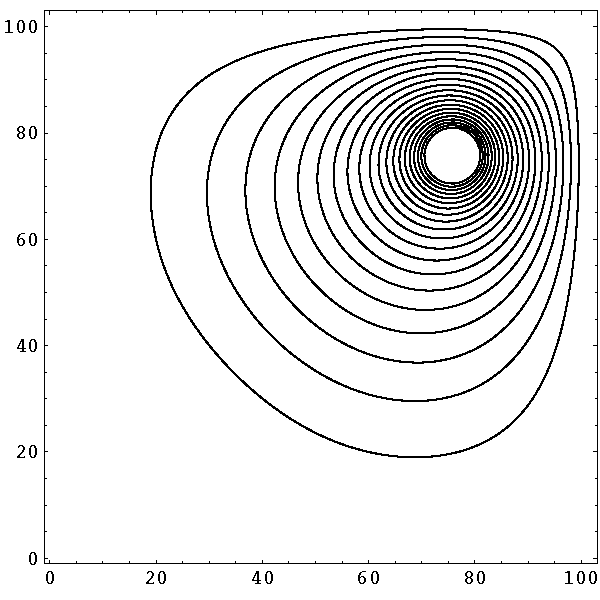
\includegraphics[width=0.8\hsize]{../common/graphics/neilcontour}
\end{center}
\caption{Niveaulinien\label{neilcontour}}
\end{figure}
\begin{figure}
\begin{center}
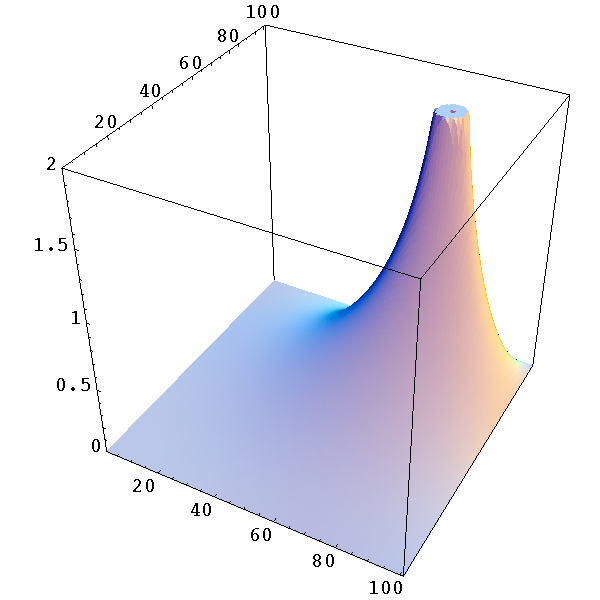
\includegraphics[width=0.8\hsize]{../common/graphics/neilloesung}
\end{center}
\caption{Potentialfläche\label{neilloesung}}
\end{figure}
Dieses Beispiel illustriert, wie die Ideen dieses Kapitels verwendet werden können,
um bessere numerische Lösungen einer partiellen Differentialgleichung
zu erhalten.

{\parindent 0pt
\medskip
{\bf Aufgabe:} Eine elektrisch leitende rechteckige Platte wird am Rand und bei 
einem Punkt $x_0\in\mathbb R^2$ im Inneren mit den Polen einer Batterie verbunden. Berechnen
Sie in jedem Punkt $x$ der Platte die Spannung gegenüber dem Rand.

\medskip
}
Das gesuchte Potential $u(x,y)$ ist eine Lösung der Gleichung
\[
\Delta u=\delta(x-x_0)
\]
mit den Randwerten
\[
u(x)=0.
\]
Direkte numerische Berechnung der Lösung wäre in der Umgebung des Punktes
$x_0$ äusserst ungenau. Motiviert von der in diesem Kapitel entwickelten
Theorie wählen wir folgendes vorgehen. Die Funktion $\sigma(x,x_0)$
ist eine harmonische Funktion mit 
\[
\Delta\sigma(x,x_0)=\delta(x-x_0)
\]
sie ist also bis auf die nicht passenden Randwerte eine Lösung.
Eine korrekte Lösung erhält man daher, in dem man das Randwertproblem
\begin{align*}
\Delta h(x)&=0&&x\in\Omega\\
h(x)&=\sigma(x,x_0)&&x\in\partial\Omega
\end{align*}
löst, was mit gängigen Programmen sehr effizient möglich ist.
Die Funktion 
\[
u(x)=\sigma(x,x_0)-h(x)
\]
ist eine Lösung. Die Lösung und die zugehörigen Niveaulinien
sind in den Abbildungen \ref{neilloesung} und \ref{neilcontour} dargestellt.

